\documentclass{article}

\def\ParSkip{} 
% Packages
\usepackage{amssymb,amsmath,amsthm,bbm}
\usepackage{verbatim,float,url,dsfont}
\usepackage{graphicx,subfigure,psfrag}
\usepackage{algorithm,algorithmic}
\usepackage{mathtools,enumitem}
\usepackage{multirow}
\usepackage{ragged2e}
\usepackage{xr-hyper}
\usepackage{array}

\usepackage[colorlinks=true,citecolor=blue,urlcolor=blue,linkcolor=blue]{hyperref}
\usepackage[margin=1in]{geometry}
\usepackage[round]{natbib}

\usepackage[utf8]{inputenc} % allow utf-8 input
\usepackage[T1]{fontenc}    % use 8-bit T1 fonts
\usepackage{booktabs}       % professional-quality tables
\usepackage{nicefrac}         % compact symbols for 1/2, etc.
\usepackage{microtype}      % microtypography

\ifdefined\TimesFont 
\usepackage{times} % use times font
\fi

\ifdefined\ParSkip 
\usepackage{parskip} % use par skip
\fi

% Theorems and such
\newtheorem{theorem}{Theorem}
\newtheorem{lemma}{Lemma}
\newtheorem{corollary}{Corollary}
\newtheorem{proposition}{Proposition}
\theoremstyle{definition}
\newtheorem{remark}{Remark}
\newtheorem{definition}{Definition}

% Assumption
\newtheorem*{assumption*}{\assumptionnumber}
\providecommand{\assumptionnumber}{}
\makeatletter
\newenvironment{assumption}[2]{
  \renewcommand{\assumptionnumber}{Assumption #1#2}
  \begin{assumption*}
  \protected@edef\@currentlabel{#1#2}}
{\end{assumption*}}
\makeatother

% Widebar
\makeatletter
\newcommand*\rel@kern[1]{\kern#1\dimexpr\macc@kerna}
\newcommand*\widebar[1]{%
  \begingroup
  \def\mathaccent##1##2{%
    \rel@kern{0.8}%
    \overline{\rel@kern{-0.8}\macc@nucleus\rel@kern{0.2}}%
    \rel@kern{-0.2}%
  }%
  \macc@depth\@ne
  \let\math@bgroup\@empty \let\math@egroup\macc@set@skewchar
  \mathsurround\z@ \frozen@everymath{\mathgroup\macc@group\relax}%
  \macc@set@skewchar\relax
  \let\mathaccentV\macc@nested@a
  \macc@nested@a\relax111{#1}%
  \endgroup
}
\makeatother

% Min and max 
\DeclareMathOperator*{\argmin}{argmin}
\DeclareMathOperator*{\argmax}{argmax}
\DeclareMathOperator*{\minimize}{minimize}
\DeclareMathOperator*{\maximize}{maximize}
\DeclareMathOperator*{\find}{find}
\DeclareMathOperator{\st}{subject\,\,to}

% Other operators
\DeclareMathOperator{\Cov}{Cov}
\DeclareMathOperator{\Var}{Var}
\DeclareMathOperator{\dm}{dim}
\DeclareMathOperator{\col}{col}
\DeclareMathOperator{\row}{row}
\DeclareMathOperator{\nul}{null}
\DeclareMathOperator{\rank}{rank}
\DeclareMathOperator{\nuli}{nullity}
\DeclareMathOperator{\spa}{span}
\DeclareMathOperator{\sign}{sign}
\DeclareMathOperator{\supp}{supp}
\DeclareMathOperator{\diag}{diag}
\DeclareMathOperator{\aff}{aff}
\DeclareMathOperator{\conv}{conv}
\DeclareMathOperator{\dom}{dom}
\DeclareMathOperator{\tr}{tr}
\DeclareMathOperator{\df}{df}

% Other shortcuts 
\def\R{\mathbb{R}}
\def\C{\mathbb{C}}
\def\E{\mathbb{E}}
\def\P{\mathbb{P}}
\def\T{\mathsf{T}}
\def\half{\frac{1}{2}}
\def\df{\mathrm{df}}
\def\hy{\hat{y}}
\def\hf{\hat{f}}
\def\hmu{\hat{\mu}}
\def\halpha{\hat{\alpha}}
\def\hbeta{\hat{\beta}}
\def\htheta{\hat{\theta}}
\def\indep{\perp\!\!\!\perp}
\def\th{^{\textnormal{th}}}

\def\cA{\mathcal{A}}
\def\cB{\mathcal{B}}
\def\cD{\mathcal{D}}
\def\cE{\mathcal{E}}
\def\cF{\mathcal{F}}
\def\cG{\mathcal{G}}
\def\cK{\mathcal{K}}
\def\cH{\mathcal{H}}
\def\cI{\mathcal{I}}
\def\cL{\mathcal{L}}
\def\cM{\mathcal{M}}
\def\cN{\mathcal{N}}
\def\cP{\mathcal{P}}
\def\cS{\mathcal{S}}
\def\cT{\mathcal{T}}
\def\cW{\mathcal{W}}
\def\cX{\mathcal{X}}
\def\cY{\mathcal{Y}}
\def\cZ{\mathcal{Z}}

\usepackage[normalem]{ulem}
\usepackage{centernot}

\title{Lecture 3: Regression and Smoothing \\ \smallskip  
\large Introduction to Time Series, Fall 2023 \\ \smallskip
Ryan Tibshirani}
\date{}

\begin{document}
\maketitle
\RaggedRight
\vspace{-50pt}

Related reading: Chapters 2 of Shumway and Stoffer (SS); Chapter 7 of Hyndman
and Athanasopoulos (HA).   

\section{Simple regression}

\subsection{Population version}

\begin{itemize}
\item We'll start off by learning the very basics of linear regression, assuming
  you have not seen it before. A lot of what we'll learn here is not necessarily
  specific to the time series setting, though of course (especially as the
  lecture goes on) we'll emphasize the time series angle as appropriate

\item A \emph{simple linear regression} model for a response variable $y$ and
  predictor (or covariate, or feature) variable $x$ is one in which we seek
  \emph{coefficients} (or parameters) $\beta_0$ and $\beta_1$, such that,
  informally,  
  \[
  y \approx \beta_0 + \beta_1 x
  \]
  To be clear, here $x,y$ are all real-valued (rather than multivariate) random
  variables 

\item If we had access to the full distributions of $x,y$, which is what we call
  the ``population version'' of regression, then we could ask: what is the best
  choice of parameters $\beta_0,\beta_1$ with respect to expected squared error?  

\item Mathematically, we are looking to solve
  \begin{equation}
  \label{eq:ls_pop}
  \min_{\beta_0, \beta_1} \, \E\big[ (y - \beta_0 - \beta_1 x)^2 \big]
  \end{equation}
  or in other words, we are asking for the ``line of best fit'' at the
  population level. You'll often also hear this referred to as the ``least
  squares'' problem

\item We can find the answer by differentiating the loss $Q = \E[ (y - \beta_0 -
  \beta_1 x)^2]$ in \eqref{eq:ls_pop} with respect to each parameter and
  setting it equal to zero. Differentiating inside the expectation gives:  
  \begin{gather*}
  \frac{\partial Q}{\partial \beta_0} = \E\big[ 2(\beta_0 + \beta_1 x - y) 
  \big] = 0 \\ 
   \frac{\partial Q}{\partial \beta_1} = \E\big[ 2x (\beta_0 + \beta_1 x - y)
   \big] = 0  
  \end{gather*}
 
\item As you'll show on the homework, solving this pair of equations gives the 
  \emph{population regression coefficients}:
  \begin{equation}
  \label{eq:coef_pop}
  \beta^*_1 = \frac{\Cov(x, y)}{\Var(x)}, \quad 
  \beta^*_0 = \E(y) - \beta^*_1 \E(x)
  \end{equation}

\item Recalling that \smash{$\Cor(x, y) = \Cov(x, y) / \sqrt{\Var(x) \Var(y)}$}, 
  we may rewrite the slope as 
  \[
  \beta^*_1 = \Cor(x, y) \sqrt{\frac{\Var(y)}{\Var(x)}},
  \]
  which shows that it treats $x,y$ \emph{asymmetrically}. This is important to
  remember. In general, when $y$ is the response and $x$ is the predictor, we 
  speak this relationship as the ``regression of $y$ on $x$''
\end{itemize}

\subsection{Sample version}

\begin{itemize}
\item For the ``sample version'' of linear regression, we seek $\beta_0,\beta_1$
  such that for given samples $x_i,y_i$ (covariate and response pairs), $i =
  1,\dots,n$,  
  \[
  y_i \approx \beta_0 + \beta_1 x_i, \quad i = 1,\dots,n
  \]
  but without access to the full distributions of each $x_i$ and $y_i$, just
  given these samples

\item We can imagine two ways to proceed:
  \begin{enumerate}
  \item Start from the population-level formula \eqref{eq:coef_pop}, and use 
    plug-in estimates for the covariance and variance
\item Start from the population-least least squares problem \eqref{eq:ls_pop},
  write down a sample version, then solve it
  \end{enumerate}

\item Somewhat remarkably, these two strategies end up at the same answer
  (which need not be the case)

\item For strategy 1, we use the sample covariance and sample variance, 
  \[
  \widehat{\Cov}(x,y) = \frac{1}{n} \sum_{i=1}^n (x_i - \bar{x}) (y_i -
  \bar{y}), \quad
  \widehat{\Var}(x) = \frac{1}{n} \sum_{i=1}^n (x_i - \bar{x})^2
  \]
  where \smash{$\bar{x} = \frac{1}{n} \sum_{t=1}^n x_t$} and \smash{$\bar{y} =
    \frac{1}{n} \sum_{i=1}^n y_i$} are the sample means, and plug these into
  \eqref{eq:coef_pop} to get:  
  \begin{equation}
  \label{eq:coef}
  \hbeta_1 = \frac{\sum_{i=1}^n (x_i - \bar{x}) (y_i - \bar{y})} 
  {\sum_{i=1}^n (x_i - \bar{x})^2}, \quad 
  \hbeta_0 = \bar{y} - \hbeta_1 \bar{x}
  \end{equation}
  which we call the \emph{sample regression coefficients}

\item For strategy 2, we write down the sample least squares problem   
  \begin{equation}
  \label{eq:ls}
  \min_{\beta_0, \beta_1} \, \sum_{i=1}^n (y_i - \beta_0 - \beta_1 x_i)^2 
  \end{equation}
  
\item Similar to before, denote the loss in \eqref{eq:ls_pop} by \smash{$Q =
    \sum_{i=1}^n (y_i - \beta_0 - \beta_1 x_i)^2$} and differentiate with
    respect to each parameter and set it equal to zero:
  \begin{gather*}
  \frac{\partial Q}{\partial \beta_0} =  \sum_{i=1}^n 2(\beta_0 + \beta_1 x_i -
  y_i) = 0 \\ 
   \frac{\partial Q}{\partial \beta_1} = \sum_{i=1}^n  2x_i (\beta_0 + \beta_1
   x_i - y_i) = 0  
  \end{gather*}
 
\item You'll show on the homework that solving this pair of equations leads you
  right back to \eqref{eq:coef}

\item The \verb|lm()| function in R performs linear regression. The notation you
  use is \verb|lm(y ~ x)|, where \verb|y ~ x| is called a ``formula''. This can
  be read as an instruction: ``regress $y$  on $x$''    

\item Figure \ref{fig:chicken} gives an example where we regress chicken
  prices---our response, $y$, on time---our predictor $x$. Just to give you a
  clear sense, the data are
  \begin{gather*}
  y_1 = 65.58, \, y_2 = 66.48, \, y_3 = 65.70, \dots \\
  x_1 = 2001.583, \, x_2 = 2001.667, \, x_3 = 2001.750, \dots
  \end{gather*}
  where we interpret each value of $x$ as a given year plus a fraction,
  representing the month of the year
  
\item After running \verb|lm()|, the resulting object is a (special) list, with
  a lot of useful  components. Calling \verb|coef()| on the object gives the
  regression coefficients   

\item Figure \ref{fig:cardio} gives another example, of a different flavor. Now
  the response $y$ is itself one time series: cardiovascular mortality in Los
  Angeles over a certain time period, and the covariate $x$ is itself another
  time series: particulate levels in Los Angeles over the same time period. The 
  top panel in Figure \ref{fig:cardio} plots them individually as time series,
  and the bottom panel plots them together, as a scatter plot, toether with the
  fitted line from linear regression. We can imagine, in a future period (beyond
  the end date of these time series), using the estimated regression
  coefficients to predict mortality from particulate 
  levels  
\end{itemize}

\begin{figure}[tb]
\centering
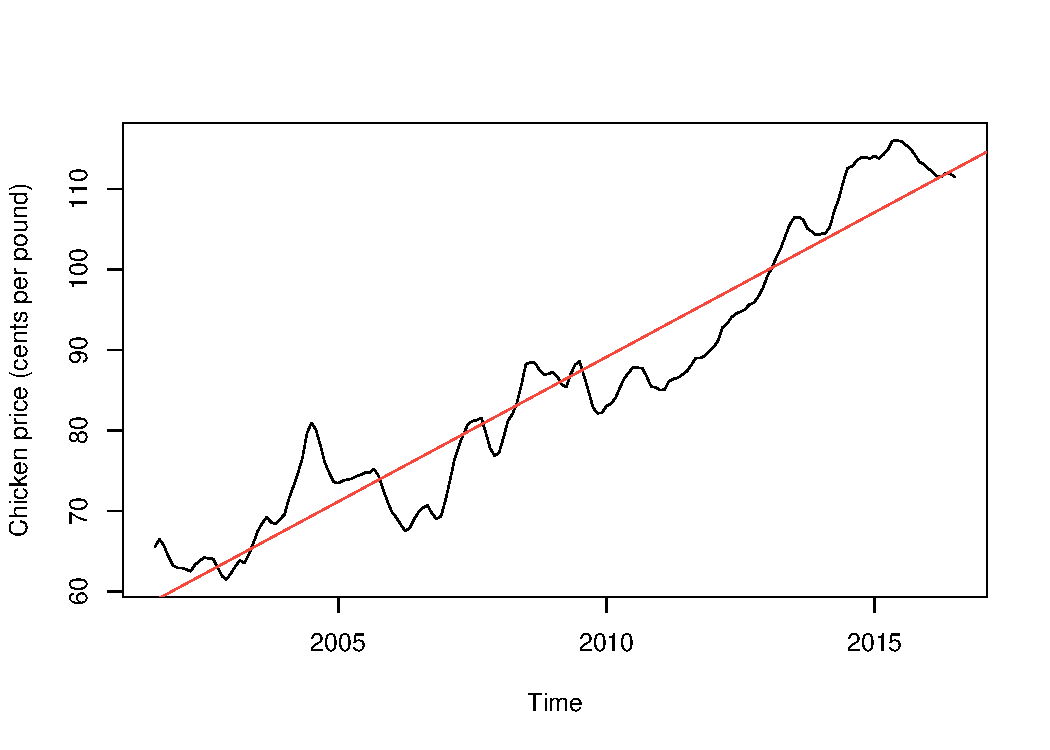
\includegraphics[width=0.875\textwidth]{fig/chicken-1.pdf}
\caption{\it Linear regression of chicken prices and on time (from SS).} 
\label{fig:chicken}
\end{figure}

\begin{figure}[p]
\centering
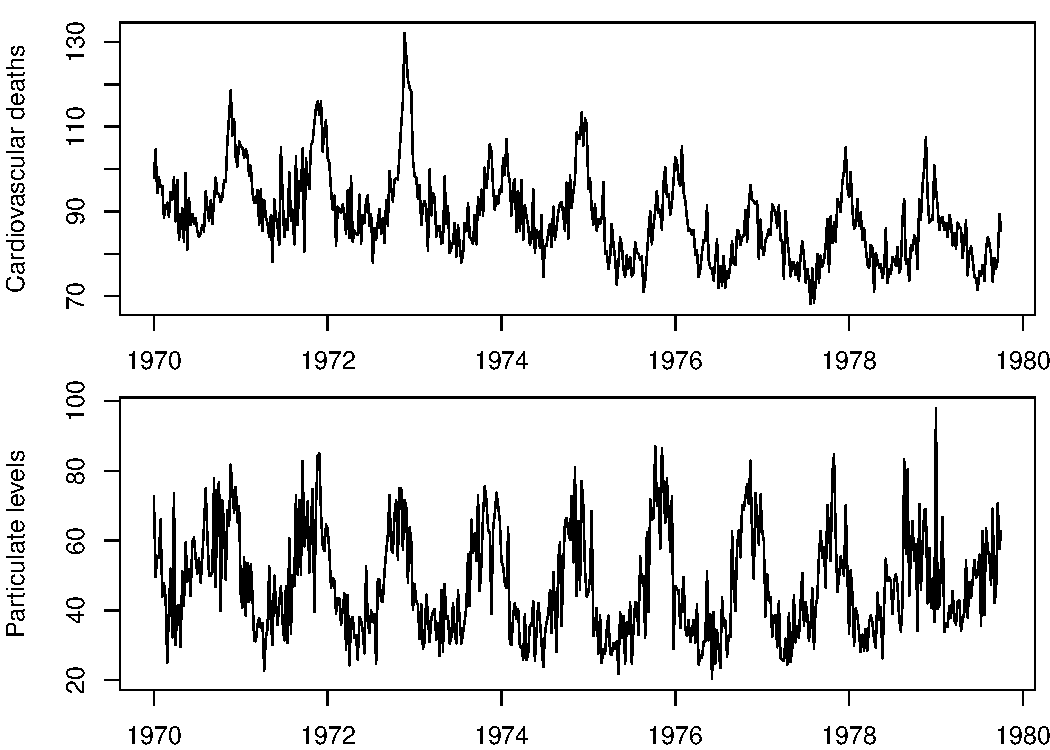
\includegraphics[width=0.875\textwidth]{fig/cardio-1.pdf} 

\bigskip\bigskip
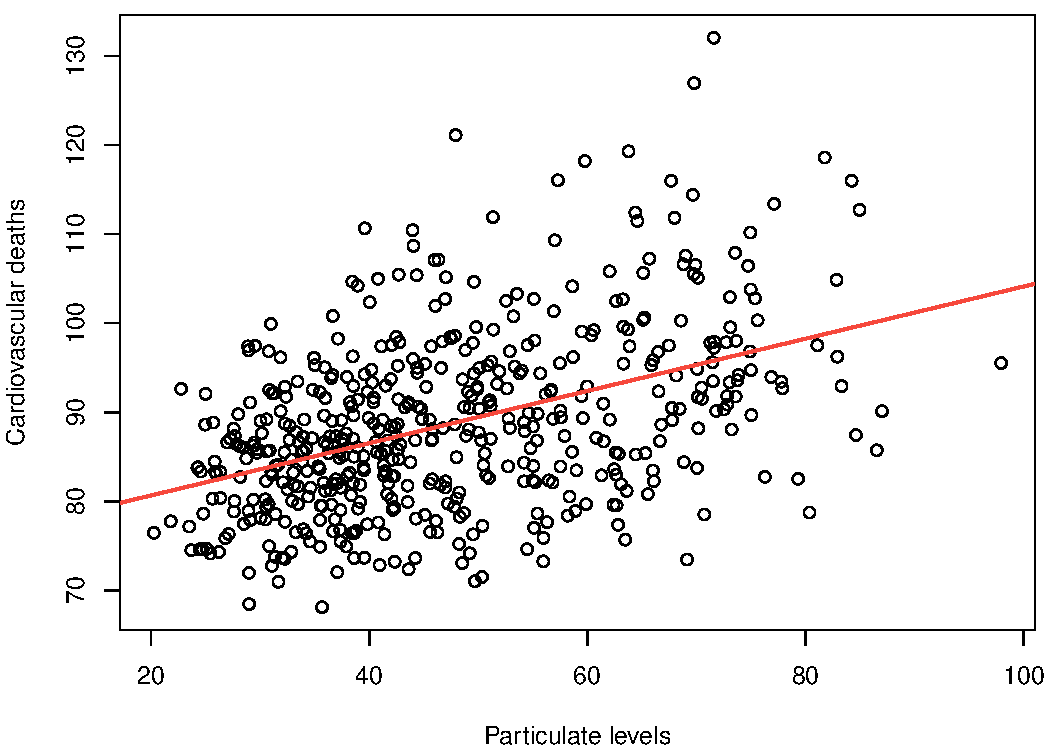
\includegraphics[width=0.875\textwidth]{fig/cardio-2.pdf}
\caption{\it Linear regression of cardiovascular mortality on particulate levels 
  in Los Angeles (from SS).} 
\label{fig:cardio}
\end{figure}

\subsection{Prediction: ex-ante and ex-post}

\begin{itemize}
\item We can use the estimated coefficients  \smash{$\hbeta_0, \hbeta_1$} in
  \eqref{eq:coef} from linear regression estimates to make \emph{predictions}
  about the response given a new predictor value $x_{\text{new}}$. This
  prediction is  
  \[
  \hat{y}_{\text{new}} = \hbeta_0 + \hbeta_1 x_{\text{new}},
  \]
  where the ``hat'' notation on the left-hand side emphasizes that it is an not  
  observed, but an estimated (predicted) value of the response

\item In time series context, we often will use the term \emph{forecasting}
  synomously with \emph{prediction}. In the time series, there is an interesting
  distinction between two types of forecasts, based on \emph{whether or not the
    predictor value $x_{\text{new}}$ needed to make forecasts is available in
    advance}. Specifically:   
  \begin{itemize}
  \item An \emph{ex-ante forecast} is a ``true'' forecast, using only
    information that is available at the time the forecast was issued. So the
    predictor values need to either be available, or themselves be
    forecasted. For instance, we can make ex-ante forecasts in the chicken 
    regression example

  \item An \emph{ex-post forecast} is made using later information on the
    predictors. So we wait until $x_{\text{new}}$ is observed, then issue our
    forecast. For instance, we can make ex-post forecasts in the mortality
    regression example (but cannot easily make ex-ante forecasts unless we 
    somehow could forecast particular levels into the future)
  \end{itemize}

\item One way around the circumvent the potential difficulty of making ex-ante
  forecasts is to use \emph{lagged predictors}; we'll discuss this and other
  forecasting issues in more detail later
\end{itemize}

\subsection{A note on assumptions and philosophy}

\begin{itemize}
\item What have we assumed above? \emph{Nothing.} That is, \emph{we do  
    not need to assume that the true relationship between $y$ and $x$ is linear
    in order to perform linear regression as in \eqref{eq:coef}}

\item Thus, in general, there need not be any ``true regression coefficients'' 
  that we're actually tracking ... but, we can always think of the sample
  estimates \smash{$\hbeta_0, \hbeta_1$} in \eqref{eq:coef} as tracking 
  the population quantities \smash{$\beta^*_0, \beta^*_1$} in
  \eqref{eq:coef_pop}. The latter are basically also always well-defined, 
  regardless of linearity. Recall, they are the viewed as the best linear
  approximation at the population level 

\item So, to be clear, we can always fit sample coefficients \smash{$\hbeta_0,
    \hbeta_1$} and use them to make predictions (forecasting, in time
  series). Sometimes we call this our ``working model'': to use a linear working
  model is a modeling decision, not an assumption  

\item If this predicts well (has good accuracy), then our working model was a
  good decision, and depending on our use case, we may not even care about
  whether the true model is linear (or related assumptions in classical linear
  modeling) 

\item Meanwhile, for use cases would that require \emph{inference}, we require
  lots of assumptions. More on this, later
\end{itemize}

\section{Multiple regression}

\subsection{Population version}

\begin{itemize}
\item What about the case where we have more than out covariate? This is called
  \emph{multiple linear regression}. Now let $x  = (x_1, \dots, x_p) \in \R^p$
  be a random vector of covariates, with each entry $x_j$ being an individual
  covariate of interest

\item We seek $\beta_0$, which is an intercept term as before, and also a whole 
  coefficient vector $\beta = (x_1, \dots, x_p) \in \R^p$, such that 
  \[
  y \approx \beta_0 + \underbrace{\beta_1 x_1 + \cdots + \beta_p
    x_p}_{\textstyle \begin{array}{c} \beta^\T x \end{array}}
  \]

\item Our convention throughout this class will be to \emph{treat all vectors as 
    column vectors}. Thus $a^\T$, which is the transpose of a vector $a$, is a
  row vector, and for vectors $a,b \in \R^d$, we can use $a^\T b = a_1 b_1 +
  \cdots a_d b_d$ to denote their inner product. 

\item (Note that of course $a^\T b = b^\T a$, so it doesn't matter whether we
  write $\beta^\T x$ or $x^\T \beta$ in our model)

\item As in \eqref{eq:ls_pop}, we define the population-level regression
  coefficients by minimizing expected squared error,   
  \begin{equation}
  \label{eq:ls_pop_mult}
  \min_{\beta_0, \beta} \, \E\big[ (y - \beta_0 - x^\T \beta)^2 \big]
  \end{equation}

\item The solution, which you can think of as generalizing \eqref{eq:coef_pop},
  is 
  \begin{equation}
  \label{eq:coef_pop_mult}
  \beta^* = \Cov(x)^{-1} \Cov(x, y), \quad 
  \beta^*_0 = \E(y) - \E(x)^\T \beta^*
  \end{equation}

\item  Let's check that the dimensions make sense: here $\Cov(x) \in \R^{p
    \times  p}$, a $p \times p$ matrix of real values; the element in its $i\th$
  row and $j\th$ column is   
  \[
  [\Cov(x)]_{ij} = \Cov(x_i, x_j)
  \]
  Also $\Cov(x, y) \in \R^p$, a $p$-dimensional vector, with $i\th$ entry
  \[
  [\Cov(x, y)]_i = \Cov(x_i, y)
  \]
  So $\Cov(x)^{-1} \Cov(x, y) \in \R^p$, itself a $p$-dimensional vector, which
  is what we need for $\beta^*$ in \eqref{eq:coef_pop_mult}. Similarly, you can
  check that the dimensions make sense for $\beta^*_0$ 

\item To derive \eqref{eq:coef_pop_mult} as the minimizer in
  \eqref{eq:ls_pop_mult}, we can again differentiate with respect to each
  $\beta_j$ and set the result to zero, but the calculation is a little more
  difficult (maybe it'll be a bonus on the homework) 
\end{itemize}

\subsection{Sample version}

\begin{itemize}
\item The sample version of multiple linear regression falls out of the 
  population version entirely analogously, as it did in the simple linear
  regression case. We seek $\beta_0 \in \R$ and $\beta_1 \in \R^p$ 
  such that for given samples $x_i,y_i$ (covariate and response pairs), $i =
  1,\dots,n$,  
  \[
  y_i \approx \beta_0 + \underbrace{\beta_1 x_{i1} + \cdots + \beta_p 
    x_{ip}}_{\textstyle \begin{array}{c} x_i^\T \beta \end{array}}, \quad 
  i = 1,\dots,n 
  \]

\item We can do this either by plug-in estimates from \eqref{eq:coef_pop_mult},
  or by writing down a sample version of the least squares problem
  \eqref{eq:ls_pop_mult} and solving it, and again they will both lead to the 
  same answer

\item Let's pursue the latter. It will be convenient to adopt the following
  convention, which alleviates us from keeping track of an explicit intercept 
  term $\beta_0$, without any loss of generality. We simply write  
  \[
  y_i \approx x_i^\T \beta, \quad i = 1,\dots,n
  \]
  without intercept. Then all results that we will derive can be translated to
  the model with intercept via the following trick: we redefine each vector
  $x_i$ so that it has a 1 prepended to it:   
  \[
  x = (1, x_1, \dots, x_p)
  \]
  Then we read of results with this new transformation: post-transformation, the
  first entry of $\beta$ serves as the intercept, and the rest serve as the
  coefficients multiplying each $x_j$  

\item (There is another way to get rid of the intercept as well, which we'll
  learn when we connect multiple to simple linear regression a bit later, which
  may be more intuitive to some of you) 

\item The sample least squares problem for multiple regression is now as
  follows:  
  \begin{equation}
  \label{eq:ls_mult1}
  \min_{\beta \in \R^p} \, \sum_{i=1}^n (y_i - x_i^\T \beta)^2 
  \end{equation}

\item The solution, obtained again by taking derivatives and setting equal to
  zero, is
  \begin{equation}
  \label{eq:coef_mult1}
  \hbeta = \bigg( \sum_{i=1}^n x_i x_i^\T \bigg)^{-1} \sum_{i=1}^n x_i y_i  
  \end{equation}

\item You can check that the dimensions all make sense here (that the right-hand
  side in \eqref{eq:coef_mult1} produces a $p$-dimensional vector)
\end{itemize}

\subsection{Matrix notation}

\begin{itemize}
\item It is more convenient, once you've sufficiently familiarized yourself with
  matrix notation, to recast regression in terms of matrices and vectors. Let $y 
  = (y_1, \dots, y_n) \in \R^n$ be the vector of our response values, and $X \in
  \R^{n \times p}$ the matrix of our predictor vectors, whose $i\th$ row is
  $x_i^\T$    

\item In other words,
  \[
  y = \begin{bmatrix} 
    y_1 \\ y_2 \\ \vdots \\ y_n 
  \end{bmatrix}, \quad 
  X = \begin{bmatrix} 
    x_{11} & x_{12} & \cdots & x_{1p} \\
    x_{21} & x_{22} & \cdots & x_{2p} \\
    \vdots & & & \\
    x_{n1} & x_{n2} & \cdots & x_{np} 
    \end{bmatrix}
  \]

\item Recall, for a coefficient vector $\beta \in \R^p$, the matrix-vector
  product $X \beta \in \R^n$, which to emphasize is an $n$-dimensional vector,
  is    
  \[
  X \beta = 
  \begin{bmatrix} 
    x_1^\T \beta \\ x_2^\T \beta \\ \vdots \\ x_n^\T \beta 
  \end{bmatrix}
  \]
  This means that we can write our sample working model compactly as
  \[
  y \approx X \beta
  \]

\item Recall, the Euclidean norm $\|\cdot\|$ of a vector $a \in \R^d$ is defined
  as $\|a\|^2 = \sum_{i=1}^d a_i^2$. This means we can write our sample least
  squares problem \eqref{eq:ls_mult1} compactly as 
  \begin{equation}
  \label{eq:ls_mult2}
  \min_{\beta \in \R^p} \, \|y - X \beta\|^2
  \end{equation}

\item Finally, the sample least squares estimates \eqref{eq:coef_mult1} can 
  be written as 
  \begin{equation}
  \label{eq:coef_mult2}
  \hbeta = (X^\T X)^{-1} X^\T y  
  \end{equation}
  This form \eqref{eq:coef_mult2} is by far the more commonly-used (and
  easily-remembered) form for the least squares coefficient estimates, compared
  to \eqref{eq:coef_mult1}. You'll prove the equivalence between the two
  forms \eqref{eq:coef_mult1}, \eqref{eq:coef_mult2} on the homework 

\item Important technical note: above in \eqref{eq:coef_mult2} (also in
  \eqref{eq:coef_mult1}), we have implicitly assumed that the features---the 
  columns of $X$---are \emph{linearly independent}. This \emph{can only happen
    if $p \leq n$}, i.e., if we have no more features than samples. Otherwise,
  $X^\T X$ will not have an inverse, strictly speaking. This is not the end of
  the world and there are many interesting things to talk about (along the lines
  of regularization) when $p > n$, but it's beyond our scope right now
\end{itemize}

\subsection{Multiple vs simple: a connection}

\begin{itemize}
\item There is quite an interesting connection between multiple regression of
  $y$ on $x$ and simple regression of $y$ on each $x_j$, the latter often
  referred to as a \emph{marginal linear regression}

\begin{quote}\it
**Warning** **Warning** **Warning**

There will be a notational clash between $x_i$ as used above and $x_j$ as will
be used here. Previously, we used $x_i \in \R^p$ to refer to vector containing
all feature values for the $i\th$ sample. Here, we are going to use $x_j \in
\R^n$ to refer to the vector containing the $j\th$ feature values measured over
all samples.       

For example, suppose we have two features: apples and bananas, and we measure
the quantity of each across $n = 100$ households. Then the previous subsection
used $x_i \in \R^2$ as the number of apples and bananas in the $i\th$
household. But here we'll use $x_j \in \R^{100}$ as the number of apples (if
$j=1$) in the 100 households, or bananas (if $j=2$) in the households. Get it? 

Since the beginning of \sout{time} regression, scholars have run up against this
problem and have racked their brains for notational solutions. But there is no
real good notational solution to this. (Yes there are lots of options but all of
them have some ugliness to them.)

We'll just make to use $x_i \in \R^p$ to \emph{always} refer to all features for
the $i\th$ sample, and $x_j \in \R^n$ to \emph{always} refer to the the $j\th$
feature for all samples (and try to never mix indices). In other words, the
$i\th$ row and $j\th$ column of the feature matrix $X$, respectively. So you
just have to remember that $i$ indexes samples (rows), and $j$ indexes features
(columns). 
\end{quote}

\item Now that we've gotten that important notational piece out of the way, we
  will define more quantities in order to describe the connection between
  multiple and marginal regression

\item Fix any $j$ (arbitrary). Given a single feature $x_j = (x_{1j}, \dots,
  x_{nj}) \in \R^n$, and response vector $y = (y_1, \dots, y_n) \in \R^n$, the 
  marginal (or simple) regression of $y$ on $x_j$, \emph{without intercept}, is
  a very similar formula to what you saw in \eqref{eq:coef}:
  \[
  \tilde\beta_j = \frac{\sum_{i=1}^n x_{ij} y_i}{\sum_{i=1}^n x_{ij}^2} 
  \]
  (Note: the effect of the intercept is only that it centers the values of
  $x_{ij}$ around their sample average, which you'll revisit on the homework)    

\item We can rewrite this succinctly in inner product notation as:
  \begin{equation}
  \label{eq:coef_j}
  \tilde\beta_j = \frac{x_j^\T y}{x_j^\T x_j}
  \end{equation}

\item Meanwhile, let's consider the $j\th$ estimated regression coefficient
  $\hbeta_j$ from the multiple regression of $y$ on $X$, as in
  \eqref{eq:coef_mult2}. Is this the same? That is, is the $j\th$ component of
  \eqref{eq:coef_mult2} the same as \eqref{eq:coef_j}? 

\item The answer is generally no! Putting in other features into the linear
  regression will generally affect the estimated coefficient for $x_j$, i.e.,
  will alter its ``predictive influence'' on $y$

\item However, there is a precise connection between multiple regression and
  marginal regression. Let's write $X_{-j} \in \R^{n \times p}$ for the feature
  matrix but after dropping $x_j \in \R^n$, the $j\th$ column. Suppose we:  
  \begin{itemize}
  \item Regress $y$ on $X_{-j}$ (a regression of $y$ on all but the $j\th$
    feature), yielding an estimated coefficient vector \smash{$\halpha \in
      \R^{p-1}$}, and residual  
    \begin{equation}
    \label{eq:resid_y}
    \hat{y}^{-j} = y - X_{-j} \, \halpha 
    \end{equation}

  \item Regress $x_j$ on $X_{-j}$ (a regression of $x_j$ on all of the other
    features), yielding an estimated coefficient vector \smash{$\htheta \in 
      \R^{p-1}$}, and residual  
    \begin{equation}
    \label{eq:resid_j}
    \hat{x}^{-j}_j = x_j - X_{-j} \, \htheta 
    \end{equation}
  \end{itemize}

\item In these residuals \eqref{eq:resid_y}, \eqref{eq:resid_j}, we have
  ``regressed out the influence'' of all other features on each of $y$ and
  $x_j$. Then, after removing such infuence, if we perform a marginal regression
  of \smash{$\hat{y}^{-j}$} on \smash{$\hat{x}^{-j}_j$}, we get precisely the
  $j\th$ multiple regression coefficient: 
  \begin{equation}
  \label{eq:coef_j_mult}
  \hbeta_j = \frac{(\hat{x}^{-j}_j)^\T\hat{y}^{-j}}
  {(\hat{x}^{-j}_j)^\T\hat{x}^{-j}_j} 
  \end{equation}

\item In other words, \eqref{eq:coef_j_mult} connects multiple regression to
  marginal regression: it shows that the $j\th$ coefficient in a multiple
  regression \eqref{eq:coef_mult2} is equivalent to a marginal regression of $y$
  on $x_j$, but only after we have accounted for the effects of all the other
  predictors, by ``regressing them out'' 

\item The best way to understand the relationship between \eqref{eq:coef_j_mult}
  and \eqref{eq:coef_mult2} is geometrically (which is also a great way to view 
  linear regression in general) but that perspecive requires a bit more advanced
  linear algebra, which we won't cover. For now, you can just think of the
  following: the bigger the \emph{correlations} between $x_j$ and columns of
  $X_{-j}$, the bigger the effect will be in \eqref{eq:resid_j}, where we
  regress out $X_{-j}$ from $x_j$, and this will make the multiple
  \eqref{eq:coef_j_mult} and marginal \eqref{eq:coef_j} coefficients quite 
  different from each other

\item On the other hand, when $x_j$ is uncorrelated with each column of
  $X_{-j}$, then the residual \smash{$\hat{x}^{-j}_j$} in \eqref{eq:resid_j} is
  no different from $x_j$, and in fact one can show that the multiple regression
  coefficient in \eqref{eq:coef_j_mult} and the marginal one in
  \eqref{eq:coef_j} are exactly the same

\item Figure \ref{fig:cardio_mult} revisits the cardiovascular mortality example
  from earlier. Now we perform the regression of cardiovascular mortality on two
  features: particulate levels and temperature. (In R we can regress \verb|y| on
  two features \verb|x1| and \verb|x2| by running \verb|lm(y ~ x1 + x2)|.) For
  each feature, the coefficients from multiple regression aren't too different
  from the marginal regression coefficients (as is seen in the bottom panel by
  the slopes of the lines), though the intercept changes noticeably. The 
  relatively small change in the coefficients on particulate levels and
  temperature is due to the fact that these two are not very correlated (as is
  seen by looking at their time series, which are a bit ``out of phase'' with
  each other) 
\end{itemize}

\begin{figure}[p]
\centering
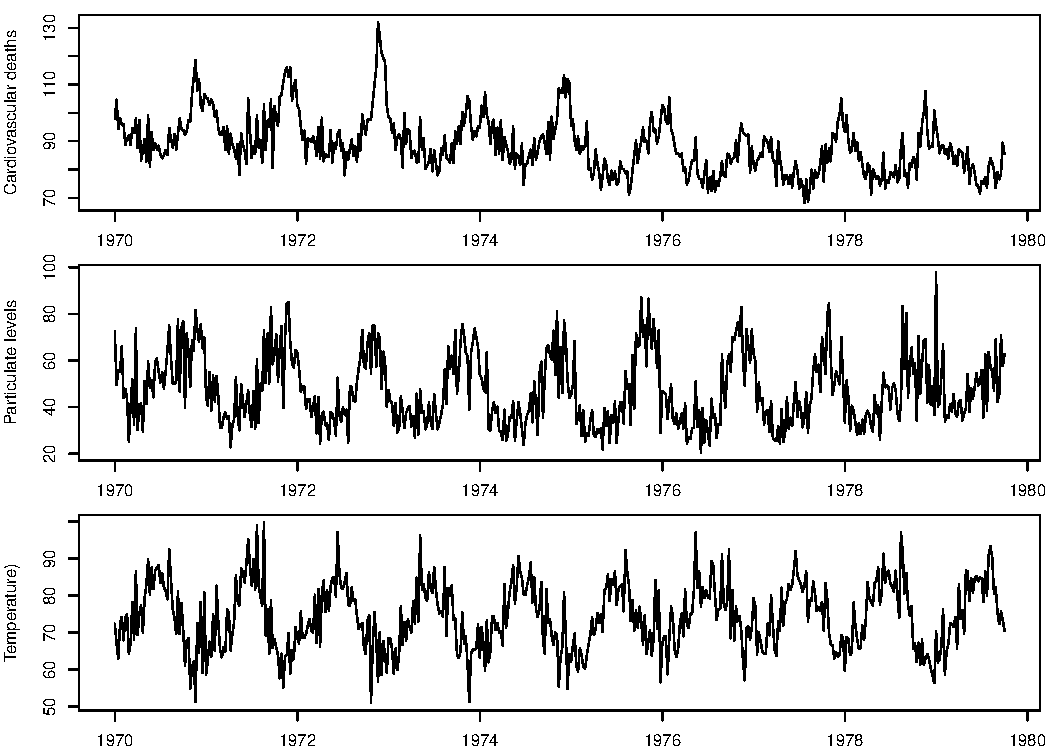
\includegraphics[width=0.875\textwidth]{fig/cardio-3.pdf} 

\bigskip\bigskip
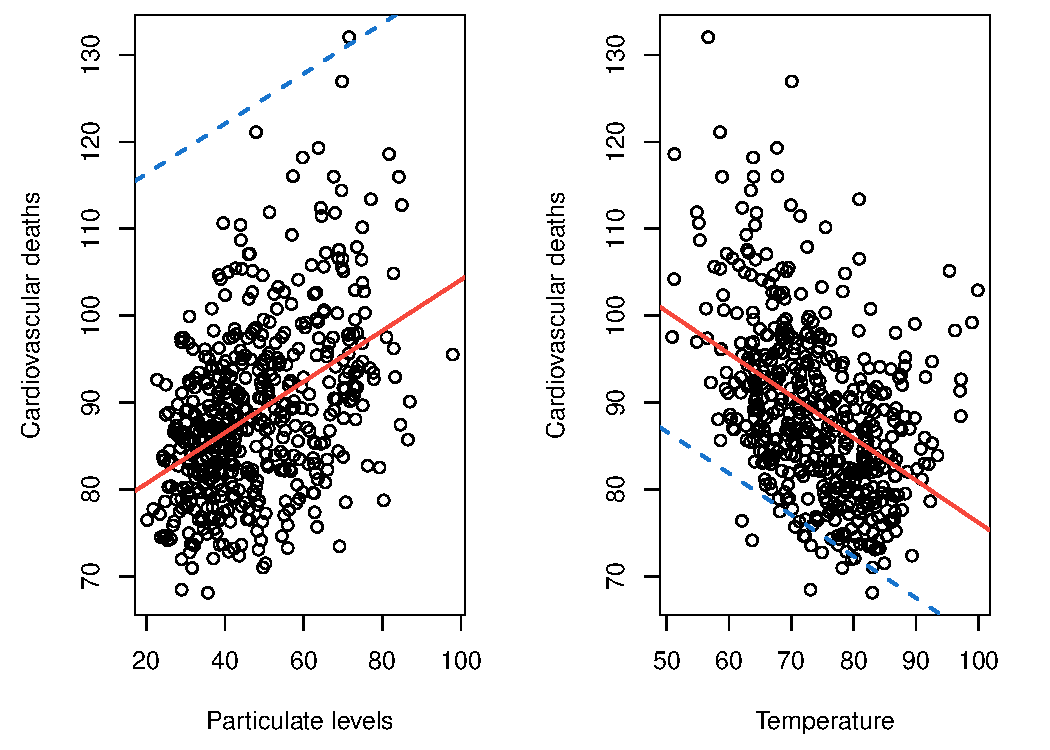
\includegraphics[width=0.875\textwidth]{fig/cardio-4.pdf}
\caption{\it Linear regression of cardiovascular mortality on particulate levels
  and temperature (this is multiple regression, with two features) in Los
  Angeles (from SS). The solid red lines denote the estimates from marginal
  regression; the dashed blue from multiple regression.} 
\label{fig:cardio_mult}
\end{figure}

\subsection{Interlude: best linear unbiased estimator}

\def\WN{\mathrm{WN}}
\def\MSE{\mathrm{MSE}}

\begin{itemize}
\item Briefly, we discuss an important optimality property here of least squares
  estimates, before moving on to classical inferential results next. We are
  going to need to introduce an assumption for this part: we assume that the
  response vector $y \in \R^n$ is related to the feature matrix $X \in \R^{n
    \times p}$ by
  \begin{equation}
  \label{eq:model}
  y = X \beta + \epsilon, \quad \text{where $\epsilon \sim \WN(0, \sigma^2 I)$}   
  \end{equation}
  for some unknown coefficient vector $\beta \in \R^p$, and a white noise vector 
  $\epsilon \in \R^n$

\item In \eqref{eq:model}, $\epsilon \sim WN(0, \sigma^2 I)$ is our notation for
  a white noise vector: the first argument specifies that the mean is zero,
  $\E(\epsilon) = 0$, and the second argument specifies that the covariance
  satisfies $\Cov(\epsilon) = \sigma^2 I$, where $I$ is the $n \times n$
  identity matrix. That is, the components satisfy $\Var(\epsilon_i) = \sigma^2$
  and $\Cov(\epsilon_i, \epsilon_j) = 0$ whenever $i \not= j$

\item Importantly, in \eqref{eq:model}, the feature matrix $X$ is assumed to be
  \emph{fixed} (not random). Therefore, we can also write \eqref{eq:model} even
  more compactly as
  \[
  y \sim \WN(X \beta, \sigma^2 I)
  \]
  This is a fairly strong assumption. We'll go into more why in the next section
  (when we go even further and assume normality of the error distribution), but
  for now we'll just emphasize that we are assuming that the mean of the
  response is truly linear in the features, and that the errors are
  homoskedastic---they have equal variance regardless of the feature values

\item Ok! So under the model \eqref{eq:model}, what can we say about the least
  squares estimates in \eqref{eq:coef_mult2}? First, note that these are
  \emph{unbiased} for the true coefficients $\beta$:
  \begin{align*}
  \E(\hbeta) &= \E \big[ (X^\T X)^{-1} X^\T y \big] \\
  &= (X^\T X)^{-1} X^\T \E(y) \\
  &= (X^\T X)^{-1} X^\T X \beta \\
  &= \beta
  \end{align*}

\item This implies it is unbiased for any contrast of $\beta$. This is the term 
  we sometimes give to an estimand of the form $a^\T\beta$, for an 
  arbitrary vector $a \in \R^d$. Observe, 
  \begin{align*}
  \E(a^\T \hbeta) &= a^\T \E(\hbeta)\big[ (X^\T X)^{-1} X^\T y \big] \\
  &= (X^\T X)^{-1} X^\T \E(y) \\
  &= (X^\T X)^{-1} X^\T X \beta \\
  &= \beta
  \end{align*}

\item One common way to measure the quality of an estimator is its \emph{mean
    squared error} (MSE), which for the least squares estimator \smash{$a^T
    \hbeta$} of the contrast $a^\T \beta$, is
  \[
  \MSE(a^\T \hbeta) = \E\big[ (a^\T \hbeta - a^\T \beta) \big]^2
  \]

\item To be clear, the expectation here is being taken with respect to data from
  the model \eqref{eq:model}

\item With respect to MSE, how good is the least squares estimator? It is, in a
  certain precise sense, the \emph{best}. It is both unbiased for $a^\T \beta$,
  as proved above, and also a \emph{linear} estimator as a function of $y$: we
  can write  
  \[
  a^\T \hbeta = \underbrace{(a^\T X^\T X)^{-1}
    X^\T}_{\textstyle \begin{array}{c} b^\T \end{array}} y  
  \]
  That is, $\hbeta = b^\T y$, where $b = X (X^\T X)^{-1} a$ 

% \item We could have also done this more explicitly from the equivalent
%   formulation in \eqref{eq:coef_mult1}:
%    \begin{align*}
%   a^\T \hbeta &= a^\T \bigg( \sum_{i=1}^n x_i x_i^\T \bigg)^{-1} \sum_{i=1}^n
%                 x_i y_i \\ 
%   &= \sum_{i=1}^n \underbrace{a^\T \bigg( \sum_{i=1}^n x_i x_i^\T \bigg)^{-1} 
%     x_i}_{\textstyle \begin{array}{c} b_i \end{array}} y_i 
%   \end{align*}
%   That is, $a^\T \hbeta \sum_{i=1}^n b_i y_i$, where \smash{$b_i = a^\T (
%     \sum_{i=1}^n x_i x_i^\T )^{-1} x_i$}, which is the same thing just written
%   differently 

\item Note: linearity of the estimator has nothing to do with linearity of the
  true regression model! The former (linearity of the estimator) is a statement
  about linearity in $y$, the response; the latter (linearity of the true
  regression model) is a statement about linearity in $X$, the features. There
  is a notational collision, but linearity is really referring to different
  things here 

\item Now for the main event: the \emph{Gauss-Markov theorem} tells us that
  the least squares estimator is the best linear unbiased estimator (BLUE) of
  $a^\T \beta$. In other words, for any other linear estimator $c^\T y$, such
  that $\E(c^\T y) = a^\T \beta$ (unbiasedness), we have  
  \[
  \MSE(a^\T \hbeta) \leq \MSE(c^\T y)
  \]

\item A proof of this fact follows from the geometric perspective on least
  squares, which we won't cover, but you can ask about it in office hours if you
  are curious  

\item (An interesting side note! Econometricians have been recently arguing about 
  whether or not we can drop the ``L'' from BLUE: is least squares the BUE? That
  is, is least squares the best unbiased estimator, period---best among all
  unbiased estimators, not just linear ones? The answer is ... yes, in a sense,
  but it depends on how you set up the problem, and in certain problem settings
  the only unbiased estimators are linear in $y$ anyway.\footnote{See Hansen
    (2022), ``A modern Gauss-Markov theorem'', and then P{\"o}tscher and
    Preinerstorfer (2022), ``A modern Gauss-Markov theorem? Really?'', and
    Portnoy (2022), ``Linearity  of unbiased linear model estimators'' (2022). A
    nice, gentle overview is given by Allison (2022), ``Is OLS BLUE or BUE?'', 
    \url{https://statisticalhorizons.com/is-ols-blue-or-bue/}. A masterful, but 
    much more mathematical overview is given in Lei and Wooldrige (2022), who
    also weave in important historical results that have been overlooked, and
    prove new ones as well.})
\end{itemize}

\section{Classical inference}

\subsection{Here comes the assumptions}

% \item For the ``sample version'' of linear regression, we envision having
%   multiple samples from \eqref{eq:pop_model} with white noise errors: 
% \begin{equation}
%   \label{eq:pop_model}
%   \begin{gathered}
%   y = \beta_0 + \beta_1 x + \epsilon, \\
%   \text{where} \quad \E(\epsilon) = 0, \; \Var(\epsilon) = \sigma^2
%   \end{gathered}
%   \end{equation}
%   Here $\epsilon$ is a stochastic error term, and as the model
%   \eqref{eq:pop_model} states, we assume it has mean zero and finite variance  
%   $\sigma^2$. To be clear, here $x,y,\epsilon$ are all real-valued (rather than 
%   multivariate) 

% \item We do not usually assume $\sigma^2$ is known, and the purpose is to
%   estimate the \emph{regression coefficients} (or parameters) $\beta_0$ and  
%   $\beta_1$, referred to as the intercept and slope, respectively
%   \begin{equation}
%   \label{eq:samp_model}
%   \begin{gathered}
%   y_i = \beta_0 + \beta_1 x_i + \epsilon, \quad i = 1,\dots,n \\
%   \text{where $\epsilon_i$, $i = 1,\dots,n$ is a white noise sequence}
%   \end{gathered}
%   \end{equation}

ASSUMPTIONS!
t-test
F-test
Evaluation: optimism of training error.
AIC, BIC, AICc, CV.

\section{Diagnostics}

ACF of residuals
Other than that, the classic ones??

\section{Forecasting}

\section{Smoothing}

\end{document}